\newpage \section{Evaluation}\label{sec:evaluation}

% \textit{Wie wird gemessen, welche Ergebnisse waren zu erwarten, was wurde erreicht. Warum gibt es Abweichungen, welche Probleme enthält die Messmethode.\todo{raus}}

Im folgenden Abschnitt wird die implementierte Lösung hinsichtlich der Leistungs- und Qualitätsanforderungen (vgl. Abschnitt \ref{sec:requirements}) evaluiert. Ergänzend zur Bestimmung und Beschreibung der Ergebnisse werden mögliche Probleme der Evaluation und des Systemaufbaus in Abschnitt \ref{sec:discuss} beschrieben.

Da zum Zeitpunkt der Fertigstellung der Arbeit noch kein ausreichend umfangreicher realer Datensatz zur Verfügung stand, wurde der frei verfügbare MovieLens 1M \citep{movielens1m} Datensatz genutzt. Dieser besteht aus ca. 1 Million Nutzerbewertungen von 3.900 Nutzern für 6040 Kinofilme. Für jeden Nutzer liegen zudem mindestens 20 Bewertungen vor. Der Datensatz wurde gewählt, da er bereits in zahlreichen Publikationen zur Ergebnisevaluation genutzt wird  (u.a.  \citep{Cacheda2011}, \citep{Candillier:2008}, \citep{Paterek07} und \citep{Herlocker:1999:AFP:312624.312682}) und so gute Vergleichbarkeit bei den Ergebnissen gegeben ist.

Um zudem realistische Leistungsmessungen der Suchlösung durchführen zu können, war es notwendig neben den reinen Bewertungsdaten textuelle Inhalte im zu untersuchenden Solr-Index zu speichern. Zu diesem Zweck wurde der Index auf Basis der korrespondierenden Filmdaten aus offenen Datenquellen\footnote{http://www.themoviedb.org/, http://mymovieapi.com/} gefüllt, so dass pro Film zwanzig verschiedene Textfelder u.a. mit Titel, Beschreibungen, Schauspielernamen und Stichworten zum Film gefüllt waren. Die Apache Solr Konfigurationsdateien (vgl. Abschnitt \ref{sec:solr}) sind vollständig in Anhang \ref{app:solrconfig} dokumentiert, die Skripte zur Indexing der textuellen Informationen und der zugehörigen Featurevektoren befinden sich zur besseren Nachvollziehbarkeit in einem Respository\footnote{Git Repository: https://gitorious.org/recommend/imdb-index}.

\newpage
\subsection{Ergebnisse}

\subsubsection{Leistung}\label{sec:performance}

Zur Bestimmung der Leistung wurden jeweils die in Abschnitt \ref{sec:requirements} beschriebenen Anforderungen an die Anfragen pro Sekunde für die einzelnen Dienste geprüft. Als Referenzsystem wurden mit Ubuntu Server 12.04 betriebener Server genutzt.  Die Hardware der Servers wurde mit 16 GB RAM und einem Dual-Core Intel Xeon E31275 so gewählt, dass diese mit Amazon EC2 m1.xlarge Instanzen\footnote{Amazon EC2 Instanz-Typen: http://aws.amazon.com/de/ec2/instance-types - geprüft am 13.09.2013} vergleichbar sind. Als Webserver bzw. Servlet-Container wurde Jetty\footnote{http://www.eclipse.org/jetty/} Version 8 hinter einem Nginx \gls{Reverse Proxy} genutzt.

Die Testpläne wurden mit Apache Jmeter\footnote{http://jmeter.apache.org/} aufgebaut und durchgeführt. Sie werden in einem eigenen Repository zur besseren Nachvollziehbarkeit zur Verfügung gestellt\footnote{Git Repository: Performance Tests: https://gitorious.org/recommend/performance-tests}. Um eine möglichst gleichförmige Ausführung zu gewährleisten wurden die Tests automatisch durchgeführt (vgl. Listing \ref{lst:jmeterscript}). Die einzelnen Messungen liefen, wenn nicht anders angegeben, jeweils 60 Sekunden mit einer vorgelagerten 30-sekündigen Ruhephase. Alle Systeme wurden im gleichen Rechenzentrum genutzt, um den Einfluss von Netzwerklatenzen zu vermindern.

Die vollständige Auflistung der Messergebnisse für die einzelnen Systembestandteile und Konfigurationen befindet sich in Anhang \ref{app:performance}.

 \lstinputlisting[caption=Script zur systematischen Ausführung von Leistungstests mit Apache Jmeter,language=bash,label={lst:jmeterscript}]{Listings/jmeter.txt}

\newpage

\paragraph{Tracker} Da die große Anzahl der zu erwartenden Anfragen auch eine sehr großen Zahl gleichzeitiger Verbindungen erfordert, wurden neben dem möglichen Durchsatz auch die maximal möglichen parallelen Verbindungen ermittelt. Um der normalen Nutzung des Dienstes zu entsprechen, wurden zufällige Trackingevents über die HTTP-Schnittstelle an den Dienst gesendet und die entsprechende Antwort geprüft.

Die Erwartung, dass der Dienst ab einer bestimmten Anzahl paralleler Anfragen neue Verbindungen nichtmehr annehmen kann und diese abweisen muss, wurde erfüllt. Wie in Abbildung \ref{fig:chart_tracker} deutlich wird, ist diese Schwelle bei ca. 350 gleichzeitigen Verbindungen erreicht. Dies hat zur Folge, dass der maximale Durchsatz stark einbricht- Ab ca. 600 parallelen Anfragen kommt es zu Verbindungsabbrüchen was durch die ebenfalls abgebildeten Fehlerquote gezeigt wird..

Die Anforderungen an den maximalen Durchsatz erreicht bzw. übertrifft der so betriebene Dienst. Zum Test von dauerhafter Stabilität wurden, ergänzend zu den Test der Lastspitzen, auch zwei dreißigminütige Tests mit  50 bzw. 100 Anfragen pro Sekunde durchgeführt. In beiden Tests konnten keine Fehler oder Verbindungsabbrüche gemessen werden.

\begin{figure}[htb]
  \centering
    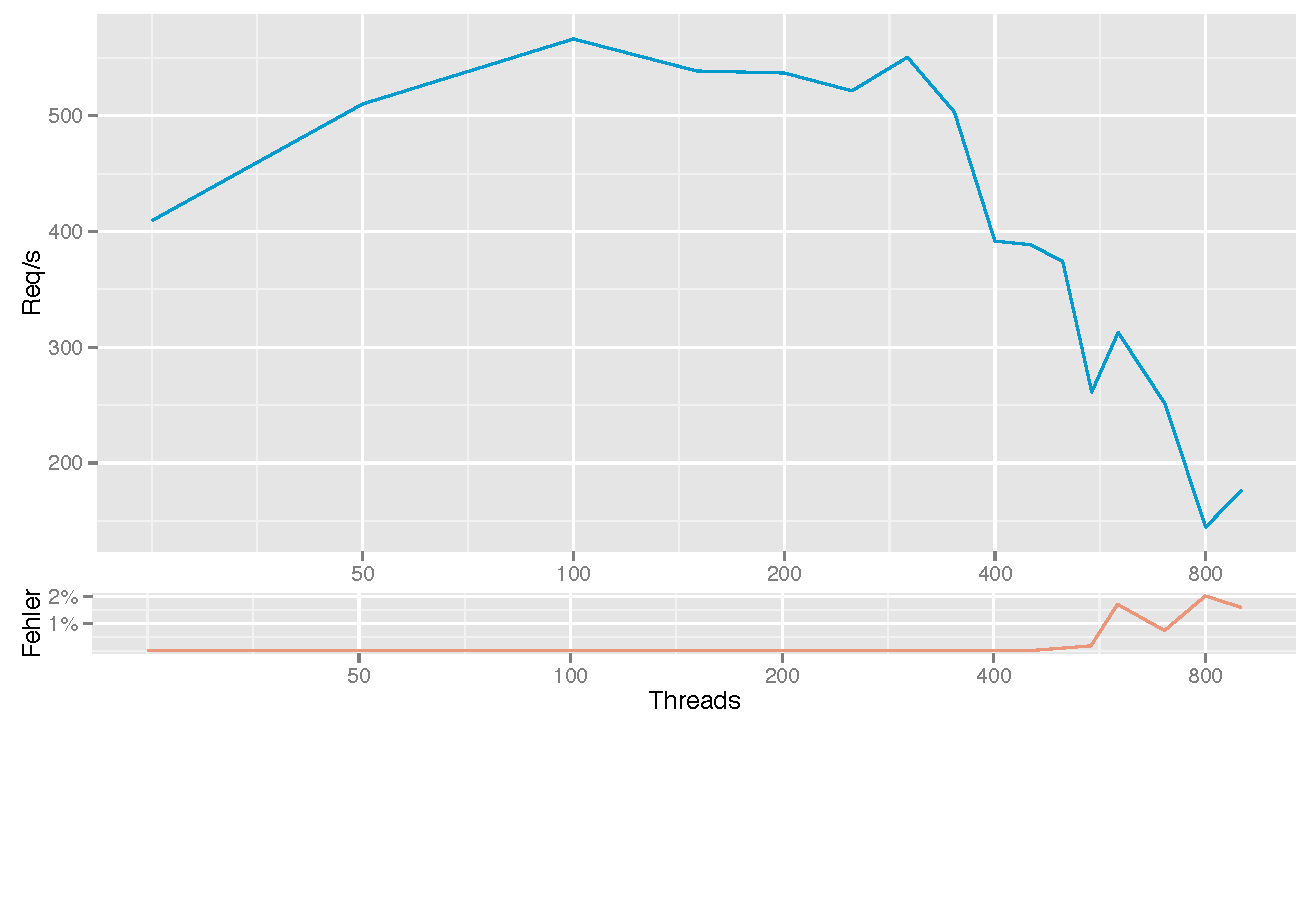
\includegraphics[width=\textwidth]{Abbildungen/tracker.pdf}
    \caption[Leistung Tracker]{Trackerleistungsdiagramm - Gegenüberstellung der Anzahl der parallel genutzten Threads, der erzielten Leistung und der Fehlerquote. { \scriptsize (eigene Darstellung)}}
    \label{fig:chart_tracker}
\end{figure}

\paragraph{Apache Solr} Zur Messung der Leistungsfähigkeit der verschiedenen Personalisierungsmethoden, wurden die Leistungswerte der Suche ohne Personaliserung mit denen der beiden Personalisierungsmethoden gegenübergestellt. Da bei großen Daten- bzw. Anfrageaufkommen die Suchanfragen wie in Abschnitt  \ref{sec:solrshards} beschrieben auch auf mehrere Backend-Server verteilt werden können, wurde die Evaluation mit bis zu drei Solr-Instanzen durchgeführt. Um eine maximale Lesegeschwindigkeit zu ermöglichen, waren die Instanzen ohne Sharding, d.h. mit voller Daten-Replikation, konfiguriert. Bei der Personalisierung mittels Webservice wurde zudem für jede Solr-Instanz ein eigener Recommendation-Service aufgesetzt. Da der Suchindex, durch den geringen Umfang der Beispieldaten, von Solr vollständig im Speicher gehalten werden kann, waren Durchsatzgrößen von 200 Requests pro Sekunde pro Solr-Instanz zu erwarten. Vergleichbare Ergebnisse werden in \citep{Rappold2013}, bei der Nutzung einer RAM-Disk, beschrieben.

Die Anfragen wurden auf Basis von zufällig gebildeten Suchausdrücken von bis zu 5 Wörtern gestellt. Die dafür verwendeten Wörter wurden so gewählt, dass deren Dokumentenfrequenz (vgl. Abschnitt \ref{tfidf}) mindestens 10 und maximal 20 betrug. Dadurch sollte sichergestellt werden, dass alle Ergebnislisten ähnlich umfangreich und nicht leer waren. Ebenso wurden die für die Personalisierung notwendigen Nutzerprofile zufällig aus zwei bis zehn Elementen gebildet. Die Vermeidung von leeren Ergebnislisten und Profilen mit nicht vorhandenen Elementen sollte dabei vor allem der besseren Vergleichbarkeit dienen.  Um mögliche Probleme sichtbar zu machen, wurden leere Ergebnislisten ebenso wie Verbindungsabbrüche als Fehler aufgezeichnet.

Abbildung \ref{fig:chart_solr} stellt die Ergebnisse der Leistungsmessung gegenüber. Wie bei der Messung der Tracker-Leistung wurden ebenfalls verschiedene Parallelitätsgrade und die damit erzielbare Leistung für die verschiedenen Konfigurationen gemessen. Die in Abschnitt \ref{sec:requirements} beschriebenen Anforderung ist als graue Linie im Diagramm kenntlich gemacht. Da diese im Vergleich zum Tracker geringer ist und damit auch die zu erwartende Anzahl paralleler Anfragen erheblich niedriger sein wird, wurden die gewählten Parallelisierungsstufen anders verteilt. Um die Auswirkungen großer Verbindungszahlen dennoch zu zeigen, wurde ebenfalls bis in den Bereich von 900 parallelen Threads gemessen.

\begin{figure}[htb]
  \centering
    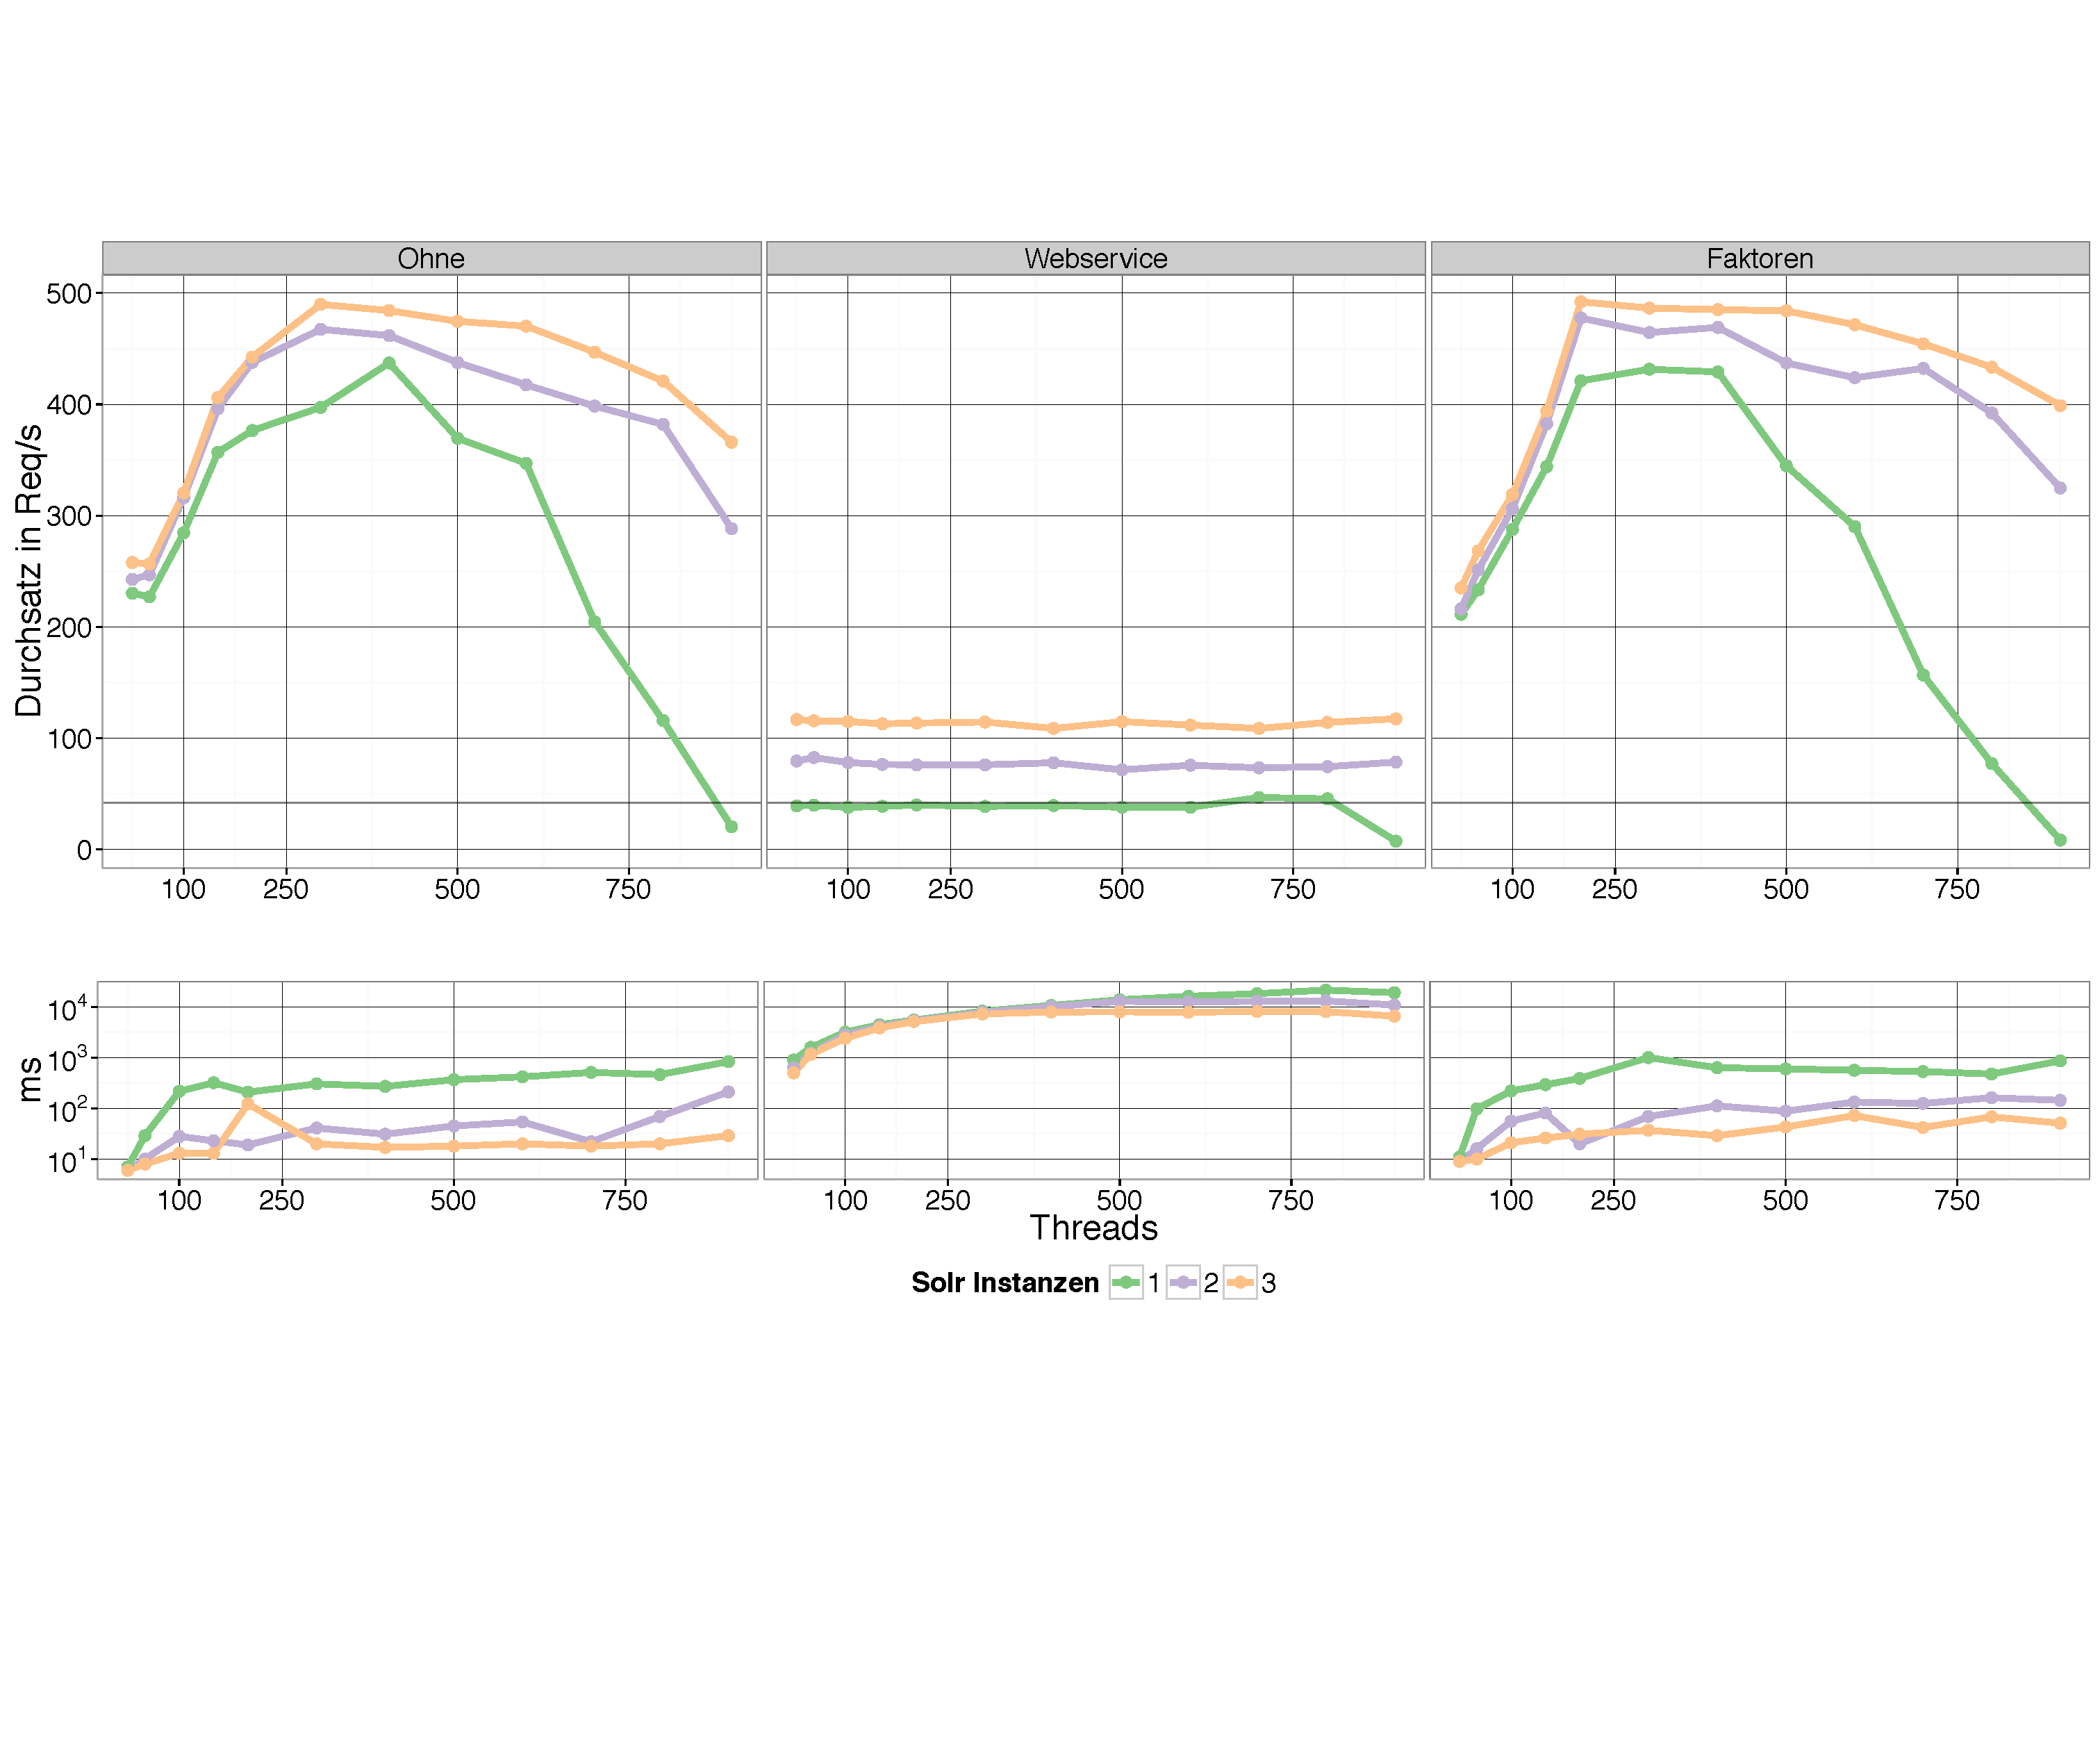
\includegraphics[width=\textwidth]{Abbildungen/personalisierung.pdf}
    \caption[Leistung d. personalisierten Suche]{Leistungsvergleich der Solr-Instanzen mit verschiedenen Personalisierungslösungen für verschiedene Parallelisierungs- und Skalierungsstufen.  {\scriptsize (eigene Darstellung)} \\ { \footnotesize \textbf{Oben}: Leistungsdaten in Requests / Sekunde -- \textbf{Unten}: 90\%-Debil der Antwortzeiten in Millisekunden.}} 
    \label{fig:chart_solr}
\end{figure}

Entgegen der Erwartung, dass die Leistung des unpersonalisierten Apache Solr mit jeder Instanz nahezu linear skaliert, zeigt sich die Auswirkung weiterer Instanzen erst bei der Steigerung der parallelen Anfragen.  Die geringe Leistung des nicht auf Parallelität optimierten Webservices spiegelt sich erwartungsgemäß in den erheblich niedrigeren Leistungswerten der entsprechenden Personalisierungslösung. Wie sich zudem zeigt, skaliert die Lösung mit weiteren Instanzen linear. Die auf Faktoren basierte Personalisierung zeigt den Erwartungen entsprechend das gleiche Skaliersungsverhalten wie die Solr-Instanzen ohne Personalisierung. Da allerdings für einige Dokumente kein Featurevektor gelernt werden konnte, zeigen die Ergebnisse eine nahezu konstante Fehlerquote von 0.3\% im Zusammenhang mit den entsprechenden Dokumenten.

Das ebenfalls in Abbildung \ref{fig:chart_solr} dargestellte 90\%-Dezil der Antwortzeiten bestätigt den deutlichen Leistungsunterschied bei der Verwendung des ausgelagerten Dienstes. 
In den gemessenen Latenzwerten zeigt sich zudem das erwartete Skalierungsverhalten bei allen Lösungen und für alle Parallelisierungsgrade.

Der zu erwartende Einbruch des Durchsatzes bei einer großen Zahl von parallelen Verbindungen zeigt sich, wie bei der Leistungsmessung des Trackers, ebenfalls. Der Schwellwert liegt zwischen 400 und 500  Verbindungen. Durch Verbindungsabbrüche hervorgerufene Fehler treten ab ca. 600 parallelen Verbindungen auf. Die in Abschnitt \ref{sec:requirements} beschriebenen Anforderungen werden von allen drei Personalisierungslösungen erreicht.

\subsubsection{Empfehlungsqualität}

Zur Messung der Qualität wurden die in Abschnitt \ref{sec:qa_rmse} beschrieben Maße zur mittleren (\acs{MAE}) und zur quadratischen (\acs{RMSE}) Abweichung genutzt. Bestimmt wurden diese für elementbasierte Nachbarschaftmodelle mit verschiedenen Distanzmetriken und für den im Rahmen der Arbeit implementierten NSVD2 Algorithmus. Als weitere Referenzwerte wurde zudem die Qualität des in Apache Mahout vorhandenen SVD-Recommenders und die eines Zufalls-Recommendes gemessen.

Das Training der evaluierten Modelle wurde mit 90\% des Datenbestandes durchgeführt. Die restlichen 10\% der Daten wurden für die Evaluation genutzt. Da es innerhalb des MovieLens 1M Datensatzes keine feste Aufteilung in Trainings- und Kontrolldaten gibt, wurde die Aufteilung zufällig vorgenommen. Um zu verhindern, dass die Aufteilung der Daten die Ergebnisse beeinflusst, wurden die Mittelwerte von 10 Berechnungen mit verschiedenen Aufteilungen für jede Methode gebildet. Die dabei gemessenen Werte sind in Tabelle \ref{tab:rmse-eval} aufgelistet.

\vfill
\begin{table}[h]
  \centering
  \begin{minipage}[b]{5in}
  \begin{tabular}{ | l | l || r | r | }
  %\cline{2}
  \hline
  \textbf { Alogrithmus } &   \textbf { Distanzmaß } &   \textbf { RMSE } &   \textbf { MAE } \\ \hline
  \multirow{4}{*}{Elementbasierte Modelle}  & Kosinus Ähnl. & 0.9730 & 0.7705 \\ 
 & Euclid. Distanz & 1.1131 & 0.8945\\   
 & Jaccard-Koeff. & 0.9616 & 0.7611 \\
 & Pearson-Korr.  & 0.9723 & 0.7553 \\ \hline
  NSVD2 & - & 	0.9840  & 0.8223 \\
  SVD &  - &	0.9062 & 0.7383 \\ \hline
  Zufall & -	&	1.7358 & 1.3689 \\ \hline
  \end{tabular}
  \caption{\footnotesize Evaluationsergebnisse der vorgestellten Recommender-Algorithmen mit Apache Mahout  (vgl. Abschnitt \ref{sec:filtermethods}). { \scriptsize (eigene Darstellung)}}
  \label{tab:rmse-eval}
\end{minipage}
\end{table}

Die auf Matrixfaktorisierung basierenden SVD und NSVD2 Modelle wurden mit 10-dimensionalen Featurevektoren trainiert. Die Laufzeit des Trainings war auf 10 Iterationen pro Feature begrenzt.

Die erzielten Ergebnisse entsprechen denen anderer Publikationen. Wie in \citep{Herlocker:1999:AFP:312624.312682} und \citep{Candillier:2008} wird bei den elementbasierten Nachbarschaftmodellen der Jaccard-Koeffizient bezüglich des \acs{RMSE} bevorzugt und die Pearson-Korrelation bezüglich des \acs{MAE}. Zudem zeigt sich, dass der Euklidische-Abstand keine geeignete Metrik für die vorliegenden Daten ist.

Der direkte Vergleich von Ergebnissen mit anderen Veröffentlichungen für die faktorenbasierten Methoden NSVD2 und SVD bezüglich der MovieLens 1M war nicht möglich. Dennoch entsprechen die erzielten Ergebnisse den Erwartungen, dass SVD bezüglich der beiden Qualitätsmaße ein besseres Ergebnis liefert als die elementbasierten Nachbarschaftsmodelle (vgl. \citep{Koren:2009:MFT:1608565.1608614}). Übereinstimmend mit den Ergebnissen aus \citep{Paterek07}, bezüglich eines anderen Datensatzens, war es ebenfalls zu erwarten, dass NSVD2 schlechtere Ergebnisse liefert.

Der Vergleich aller Ergebnisse mit denen des zufälligen Empfehlungsdienstes zeigt, dass in allen Fällen erheblich bessere Ergebnisse erzielt werden können. Da es keine quellenoffene Referenzimplementierungen des NSVD2 Algorithmus gibt, ist dieser Vergleich notwendig um einen funktionierenden aber schlecht parametrisierten von einem nicht-funktionalem Empfehlungsdienst zu unterscheiden. Da das Ziel der Qualitätstests nicht die Optimierung der Parameter für die Beispieldaten war und da sich mögliche Erkenntnisse nur begrenzt auf andere Quellen übertragen lassen, wurden keine ergänzenden Evaluationen anderer Parameterkombinationen oder mit ergänzenden Maßen (vgl. Abschnitt  durchgeführt. \ref{sec:measures}) durchgeführt.

\subsubsection{Disjunkte Kanidatenlisten} \label{sec:disjunction_check}

Zur Untersuchung der in Abschnitt \ref{sec:disjunctcanidates} beschrieben Problematik der disjunkten Ergebnislisten wurde die Größe der Schnittmenge der Ergebnislisten von Suche und Empfehlungsdienst, bei der Personalisierung mittels Webservice, untersucht. Wie in den vorangegangenen Abschnitten wurden dabei zufällige Suchen mit bis zu zwanzig Wörtern mit ebenfalls zufällig gebildeten Nutzungsprofilen betrachete. Von allen Suchergebnislisten wurden die ersten fünfzig Elemente ausgewertet und geprüft wieviele der dafür empfohlenen Elementen enthalten waren. Da zu erwarten war, dass die Größe der Schnittmenge vom Umfang der Empfehlungsliste abhängig ist, wurden vier verschiedene Größenkonfigurationen geprüft. Da die Größe der Suchergebnisliste vorwiegend davon abhängig ist, wieviele Elemente ein Nutzer sich ansehen möchte und dadurch nicht beliebig zur Konfiguration angepasst werden kann, wurde ihr Umfang nicht variiert.

Die Ergebnisse der Untersuchung werden in Abbildung \ref{fig:chart_disjunction} gegenübergestellt. Durch die zufällig gebildeten Suchbegriffe und den zudem fehlenden Kontext zum Nutzerprofil war zu erwarten, dass die Schnittmengen sehr gering sind. Diese Erwartungen wurden ebenso bestätigt wie die Annahme, dass mit zunehmendem Umfang der Empfehlungen auch die Größe der Schnittmenge steigt.

\begin{figure}[htb]
  \centering
    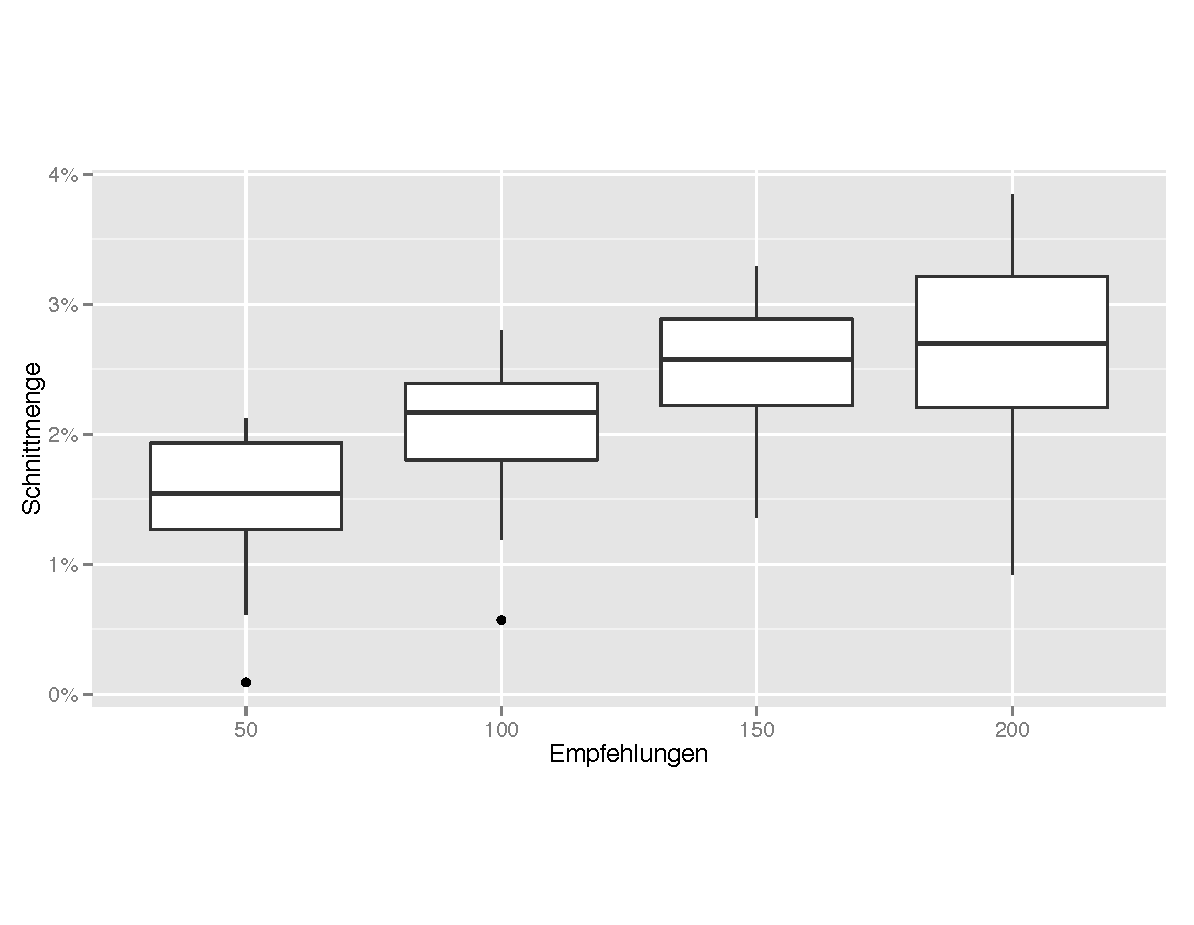
\includegraphics[width=0.75\textwidth]{Abbildungen/disjunction.pdf}
    \caption{Schnittmengenvergleich bei der Nutzung der Personalisierung mittels Webservice in Abhängigkeit der Empfehlungsgrößen {\scriptsize (eigene Darstellung)}}
    \label{fig:chart_disjunction}
\end{figure}

\subsection{Diskussion} \label{sec:discuss}

\paragraph{Skalierungsverhalten und Latenz} Da die Skalierbarkeit des Systems eines der wichtigsten Ziele der Arbeit darstellt, waren die umfassenden Tests aus Abschnitt \ref{sec:performance} notwendig und die erzielten Ergebnisse insgesamt mehr als zufriedenstellend. Die Zusammenstellung und Konfiguration der gewählten Systemkomponenten entspricht den in Abschnitt \ref{sec:requirements} beschriebenen Anforderungen. % Da alle Tests mit Standardkonfigurationen aller Bestandteile durchgeführt wurden, besteht neben den Möglichkeiten der horizontalen Skalierung ebenfalls Raum für weitere Optimierungen bezüglich der beschriebenen Plattform.

Das nicht erwartungsgemäße Skalierungsverhalten der Apache Solr-Instanzen bei geringen Parallelisierungsgraden weißt auf ein mögliches Konfigurationsproblem der Testumgebung oder des Testwerkzeuges hin. Da die Tests ausschließlich von einem einzigen Quellsystem ausgeführt wurden, ist es zum Beispiel denkbar, dass diese nicht gleichmäßig verteilt wurden bis ein gewisser Schwellwert erreicht war. Ein weiterer Faktor der in diesem Zusammenhang nicht näher untersucht werden konnte, ist die Dokumentengröße und mögliche Auswirkungen auf den erzielbaren Anfragen pro Sekunde. \citep{solrperformance} \todo{Nicht soo besonders formuliert alles}

Die erzielte mittlere Latenz des Trackers und der Suchimplementierungen entsprachen den Erwartungen. Da normale Clientsysteme in der Regel nicht im gleichen Rechenzentrum angebunden sind, entspricht die Latenz nur begrenzt den realen Bedingungen. Zudem konnte sie davon profitieren, dass die Tests auf einem einzigen System durchgeführt wurden. Da eine größere Anzahl von Clientsystemen die Verwaltung der bestehenden Verbindung und Optimierungen auf der Ebene der Transportschicht erschwert, ist im praktischem Betrieb mit deutlich höheren Latenzwerten zu rechnen. Um diese Aspekte auch in die Tests einzubeziehen, sollten die Latenzwerttests ergänzend mit einer größeren Anzahl von Clientsystemen wiederholt werden. \citep{jetty2008}

\paragraph{Apache Solr} Die erwartungsgemäß guten Leistungs- und Latenzwerte der Apache Solr-Instanzen sind bei der beschriebenen Nutzung mit wenigen tausend Dokumenten nur bedingt übertragbar. Wird die horizontale Skalierung (vgl. Abschnitt \ref{sec:sharding}) mit einer Aufteilung der Daten in verschiedene Datenblöcke pro Backend-Knoten genutzt, lässt sich das im Rahmen der Evaluation bestätigte Verhalten nur eingeschränkt übertragen. Da der Umfang der im Suchindex gehaltenen Daten mit wenigen tausend Dokumenten die vollständige Replikation auf alle drei Solr-Instanzen erlaubt und da zudem davon auszugehen ist, dass der Index jederzeit vollständige im Dokumenten-Cache von Solr vorgehalten werden konnte, entsprachen die Leistungsdaten des nicht optimierten Testsystems denen eines optimierten Produktivsystems (vgl. \citep{Rappold2013}).  Durch den geringen Umfang des Indexes konnte zudem nicht geprüft werden, inwiefern die im Solr integrierten Caches weiterhin effizient arbeiten können. Es ist zum Beispiel naheliegend, dass zwischengespeicherte Suchergebnislisten, wegen unterschiedlicher Präferenzwerte, nicht zwischen verschiedenen Nutzern übertragen werden können und so die Effizienz der Zwischenspeicher wegen der Personaliserung nichtmehr gegeben ist (vgl. \citep{solrcache}). 

%\paragraph{Systembestandteile} 
%JVM Optimierung / J2EE Container / Plattform
\paragraph{Qualitätsmaße} Da die gute Vergleichbarkeit der Empfehlungsqualität im Vordergrund stand, wurden die in den Publikationen weiter verbreiteten Fehlermaße \acs{RMSE} und \acs{MAE} genutzt. Da in der praktischen Anwendung den Top-N Ergebnissen eine sehr hohe Bedeutung zugemessen wird, kann mit diesen Maßen kein direkter Schluss, auf die Qualität eines Algorithmus in diesem Bezug, getroffen werden. Aus diesem Grund ist es sinnvoll jeden Algorithmus auch bezüglich der in Abschnitt \ref{sec:precision} beschriebenen Maße zu untersuchen. Des Weiteren sind empirische Maße (vgl. Abschnitt \ref{sec:measure_c}) für den praktischen Betrieb ein zusätzlicher wichtiger Maßstab der im Rahmen der Evaluation nicht eingeschlossen werden konnte. \citep{Cremonesi:2010:PRA:1864708.1864721}

Dass Ergebnisse und Parametrisierungen die auf dem MovieLens 1M Datensatz basieren nur unter Vorbehalt auf andere Datensätze übertragbar sind, wird in \citep{Howe08} gezeigt. Die darin gezeigten Unterschiede des \acs{MAE} waren je nach Datensatz unterschiedlich von den Parametern des Empfehlungsalgorithmuses und der Normalisierung der Daten abhängig. Ergänzend zur bedingten Übertragbarkeit der Ergebnisse, beschreibt \citep{netflix2012_2} die Abwägung bei der praktischen Implementierung eines Empfehlungsdienstes. Der möglichen Verbesserung der Empfehlungsqualität von 2-3\% bzgl. des \acs{RMSE} steht die 
Schwierigkeit einen erheblich komplexeren Algorithmus umzusetzen. So muss bei zukünftigen Implementierungen abgewogen werden zwischen der komplexeren Systemarchitektur, bei der Personalisierung mittels  Webservice, und der ggf. ungenaueren aber leistungsstärkeren Personalisierung mittels Featurevektoren.

\paragraph{Rich-gets-richer Problematik} Dass der Ausschluss der populärsten 2-5\% der Produkte zur Vermeidung des in Abschnitt \ref{sec:filterissues} beschriebenen \textbf{Richt-get-richer} Problems genutzt werden kann, wird u.a. in \citep{Cremonesi:2010:PRA:1864708.1864721} beschrieben. Ergänzend wird auch die getrennte Evaluation der Empfehlungsdienste mit und ohne die populärsten Elemente des Datensatzes vorgeschlagen. Bei der Umsetzung dieser Maßnahmen in Kombination mit der in Solr integrierten Empfehlungsbildung stellt sich allerdings das Problem, dass ein Ausschluss von Dokumenten aus dem Training auch ein Fehlen der zugehörigen Featurevektoren zur Folge hätte. In diesem Fall wäre das Auffinden der Dokumente innerhalb der personalisierten Suche auch bei relevanten Suchbegriffen nicht mehr möglich. Die Integration eines ergänzenden inhaltlichen Filters (vgl. Abschnitt \ref{rec:contentrec}) in Apache Solr erscheint hier als praktikablerer Weg der zur Wahrung des Umfangs nicht evaluiert werden konnte.

\paragraph{Disjunkte Kanidatenlisten} Da es keine Referenzwerte im Vergleich mit ähnlichen Lösungen gibt, ist eine Wertung der in Abschnitt \ref{sec:disjunction_check} beschriebenen Messergebnisse nur eingeschränkt möglich. Die gemessenen Überschneidungen von maximal 4\% machen eine umfangreiche Personalisierung der Suchergebnisse allerdings nur bedingt möglich. Die weitere Vergrößerung der Empfehlungsmenge um bessere Überschneidungswerte zu erzielen erscheint zudem sehr unrealistisch, weil damit im untersuchten Fall mehr zwischen  5- und 10\% der gesamten Elemente betrachtet werden müssten um eine erheblich geringere Zahl von Suchergebnissen zu personalisieren.

Die vorgestellten Ergebnisse, dienen aus diesem Grund vor allem dem Zweck, Vergleichswerte für spätere Anwendungsfälle aufzuzeigen. Sowohl bei der Anwendung der in Abschnitt \ref{sec:disjunctcanidates} beschriebenen Lösungsmöglichkeiten, als auch bei der praktischen Umsetzung sollten so erheblich größere Schnittmengen festzustellen sein. Eine ergänzende Evaluation ist daher über den Rahmen dieser Arbeit hinaus erforderlich.

%\paragraph{Übertragbarkeit}
%Skalierbarkeit evt. mit weiterem Datensatz ``testen'': \\
%\url{http://aws.amazon.com/datasets/6468931156960467} -> (Subset: \url{http://labrosa.ee.columbia.edu/millionsong/tasteprofile}) \\
%Signifikanz: \url{http://www.mitp.de/imperia/md/content/vmi/1634/1634_kapitel_20.pdf} \\
%Joachim05 -> Wilcoxon test
